% This must be in the first 5 lines to tell arXiv to use pdfLaTeX, which is strongly recommended.
\pdfoutput=1
% In particular, the hyperref package requires pdfLaTeX in order to break URLs across lines.

\documentclass[11pt]{article}

% Remove the "review" option to generate the final version.
%\usepackage[review]{ACL2023}
\usepackage[]{ACL2023}
\usepackage{hyperref}

% Standard package includes
\usepackage{times}
\usepackage{latexsym}
\usepackage{booktabs}
\usepackage{tabularx}
% For proper rendering and hyphenation of words containing Latin characters (including in bib files)
\usepackage[T1]{fontenc}
\usepackage{graphicx}
% For Vietnamese characters
% \usepackage[T5]{fontenc}
% See https://www.latex-project.org/help/documentation/encguide.pdf for other character sets

% This assumes your files are encoded as UTF8
\usepackage[utf8]{inputenc}


\usepackage{hyperref}
\usepackage{longtable}

% This is not strictly necessary, and may be commented out.
% However, it will improve the layout of the manuscript,
% and will typically save some space.
\usepackage{microtype}

% This is also not strictly necessary, and may be commented out.
% However, it will improve the aesthetics of text in
% the typewriter font.
\usepackage{inconsolata}


% If the title and author information does not fit in the area allocated, uncomment the following
%
%\setlength\titlebox{<dim>}
%
% and set <dim> to something 5cm or larger.

\title{NLP finale course project:Application of LLM (llama-2) to
answer Rav Questions }

% Author information can be set in various styles:
% For several authors from the same institution:
% \author{Author 1 \and ... \and Author n \\
%         Address line \\ ... \\ Address line}
% if the names do not fit well on one line use
%         Author 1 \\ {\bf Author 2} \\ ... \\ {\bf Author n} \\
% For authors from different institutions:
% \author{Author 1 \\ Address line \\  ... \\ Address line
%         \And  ... \And
%         Author n \\ Address line \\ ... \\ Address line}
% To start a seperate ``row'' of authors use \AND, as in
% \author{Author 1 \\ Address line \\  ... \\ Address line
%         \AND
%         Author 2 \\ Address line \\ ... \\ Address line \And
%         Author 3 \\ Address line \\ ... \\ Address line}

\author{Tomer shimshi \\
  %Affiliation / Address line 1 \\
  %Affiliation / Address line 2 \\
  %Affiliation / Address line 3 \\
  \texttt{tomershimshi@gmail.com} \\\And
  Amit Damri \\
  %Affiliation / Address line 1 \\
  %Affiliation / Address line 2 \\
  %Affiliation / Address line 3 \\
  \texttt{amitdamri@tau.ac.il} \\}

%\author{Tomer Shimshi 203200480     Amit Damri 313191785 }

\begin{document}
\maketitle
\begin{abstract}
In recent years the have been a increase in the popularity of LLM and theire ability to solve tasks that were considered to be above computer level such as writing a report or planing a trip abroad.
In the following paper we will apply two state of the art techniques to use an open source LLM to try and solve a problem it was not trained on and have most likely have never seen before, namely we will compare fine-tuning an LMM and  Retrieval-Augmented Generation (RAG) in order to give the LLM the ability to solve the specific task of answering a Jewish Rav question. The reason we chose this specific case is due to its Niche field which is a good way to show that if we succeed on this task we can apply the results we recive into many other fildes og life that no one tried to apply LLMs on.
In our project we found that for our specific task the RAG pipline proved more cabaple than the fine tuning approach but over all booth gave descent results.
\end{abstract}

\section{Introduction}

In the following paper we will try to use an LLM model on a specific task that it has yet to see before namely we will try to test whether a LLM is capable of answering Rav questions. For that we will first define the basic terms of the specific use case we tested in our terms of out project:
A Rav Question is question asked by a Jewish person to hes Rav , a Rav is a Jewish man who studied the Halacha laws for many years and is considered a authority in the matter, the Rav needs to answer the given question according to the Jewish tradition laws. The questions can be about anything. In the Jewish tradition it is a custom to seek guidance from your Rav about any life question you may have. If this project will succeed it can help many remote orthodox Jews  that do not have a frequent access to a near by Rav but do require answers for they're immediate questions, and since it is much more scale able to use a LLM to answer all these question rather than a real human Rav it can revolutionize the entire Jewish world.  
We know that LLMs are good with at answering questions but it is not so trivial to answer Rav Quastion and not many people are qualified to answer them.
In order to achieve this goal we will try two different approaches and try to validate which is the prefers approach:
\begin{enumerate}
    \item Model Fine tuning: fine tune an LLM on the specific task of answering Rav questions. For that we first fine tuned the model on  \href{https://www.sefaria.org.il/Kitzur_Shulchan_Arukh.1.7?lang=en}{ Kitzur Shulha Aruch} which is a book that summaries all the Jewish halacka laws and then perform a second fine tuning using a dataset we collected from the \href{https://asktherav.com/ }{Ask a Rav}) website to try and teach the model how to properly answer this type of questions.
    \item Retrieval-Augmented Generation (RAG): We used this approach in order to supply our LLMs the  \href{https://www.sefaria.org.il/Kitzur_Shulchan_Arukh.1.7?lang=en}{ Kitzur Shulha Aruch} so that it will be able to answer any question being asked according to the Halacka laws specified in the retrieval dataset
\end{enumerate}
In our project we chose to use meta \href{https://llama.meta.com/llama2/}{ llama-2 7b } model for the application of our task as it is a state of the art open source LLM.


\section{Related work}
Ever since Meta released they're open source llama-2 model there has been a lot of people from the \href{https://huggingface.co/ }{Hugging face community}) that used this open source model and fine tuned it on they're own dataset, examples for that can be found in the following guides:  \href{https://deci.ai/blog/fine-tune-llama-2-with-lora-for-question-answeringo/ }{guide No.1} or \href{https://www.confident-ai.com/blog/the-ultimate-guide-to-fine-tune-llama-2-with-llm-evaluations }{guide No.2}. And in general in the recent years fine tuning a LLM has became a lot more common. following that is what made us decide on fine tuning our llama-2 model to be able to answer Rav questions.
Although fine tuning LLMs for specific tasks have became very common in the recent years we have yet to witness a model that was trained for the specific task of answering Rav questions.

In the of Retrieval-Augmented Generation (RAG) case, recently there has been an increase in the popularity of using RAG in order to have an LLM capable of answering questions on areas it have not seen in its initial training. given that it has access to a specific dataset provided by the user.
There are many examples and guides on how to use RAG for a specific LLM  like for example 
 \href{https://www.kaggle.com/code/gpreda/rag-using-llama-2-langchain-and-chromadb/notebook#Retrieval-Augmented-Generation }{guide No.1}
 or \href{https://blog.demir.io/hands-on-with-rag-step-by-step-guide-to-integrating-retrieval-augmented-generation-in-llms-ac3cb075ab6f }{guide No.2}. even tough that RAG is increasingly more popular these days we have yet to see any example of using a RAG pipeline combined with Jewish laws in order to create a Jewish Rav capable of answering question according to the Jewish laws, so from use case point of view our work has never been tested before .
 

\begin{table}[htbp]
    \centering
    \caption{Dataset example}
    \label{tab:example}
    \begin{tabular}{ccc}
        \toprule
        question & answer   \\
        \midrule
        
        question from the site & answer from the site  \\
        
        \bottomrule
    \end{tabular}
\end{table}



\section{Training and Data collection}
\subsection{Data collection and prompt preparation}
Since all of the Rav answers are based on the Jewish laws (the halcka) we couldn't just use a question and answer dataset (as we initially taught) so we understand that the first step in creating our dataset booth for RAG and for fine tuning a pretrained model is to  first have a dataset containing the majority of the Jewish laws for that we have collected the English version of the \href{https://en.wikipedia.org/wiki/Kitzur_Shulchan_Aruch}{ Kitzur Shulhan Aruch} book since it contains most of the Jewish laws and customs while still being a relatively short text so that we can perform RAG\ fine tuning on it.
The second step for the LLM fine tuning to answer Rav question is to find the relevant dataset containaing real Rav questions and answers  and since that there is no known dataset for Rav questions we had to create a dataset ourselves.For this task we had to find a relevant site to perform data scraping from, and since most the open source models are best suited for the english language rather that the Hebrew language we performed the data scraping from an English site namely \href{https://asktherav.com/ }{Ask a Rav} site which is full of real questions and answers in English. From this site we comprised our dataset of real Rav Quaestion and answers as can be seen on table 1.
Since some of the questions\ answers on the site asked using some Hebrew words inside them (usually old Hebrew words) and since we know that the model do not handle Hebrew well we have decided to remove all these questions/ answers from the dataset, this reduced our dataset from a 1095 to 756 only English question and answers.
Here is an example of a one question and answer used in our dataset.\\
Question:\\
 May I put a frozen bag of vegetables etc. on my body on Shabbos as it might melt from my body heat?
If the answer is yes, may I cool myself off with these packets of frozen milk knowing and benefiting from the fact that they will melt? If neither of these are acceptable,may I use a cold cloth placed in the freezer?

Answer:\\

1) One may handle ice packs to cool off with, since only a small amount of water is melted, there is no intention of melting them and the melted water is going to waste. Melting ice is problematic when one actively melts it, or even when no action is taken if this his intention, for example if wants to melt it save the melted water – which is not applicable in this case.
However, frozen food items like meat and vegetables should not be used since they are muktzah.\\
2) Since you want to melt the milk, you should not purposely use it to cool off so as to proactively melt it.\\
3) Cold towels that are not wet and will not become squeezed is permissible to use\\
After we finished collection the data we needed to create the model prompt, in order for it to fit to the task at hand we created the following prompt in order to feed it into the the model : \\
you are a jewish Rav, please answer the following question according to the Halakha (Jewish law) .\\
\#\#\# Question:\\
\\
\#\#\# Answer:\\
{} EOS TOKEN\\
Where the EOS TOKEN stands for the token which the tokenizer was trained on to mark the end of sentence.
After finishing the data collection and prompt creation we loaded the model and started the model training.
\subsection{Model loading}
The model which have tested in this project is  \href{https://huggingface.co/NousResearch/Llama-2-7b-chat-hf }{meta llama-2 7B} (where the B stands for the models number of parameters in billion) As such it is are vary large model that consume a lot of RAM on the GPU in order to still be able to load and fine tune them on the provided GPU we have used \href{https://pypi.org/project/bitsandbytes/}{bitsandbytes} python library which essentially enables accessible large language models via k-bit quantization for PyTorch. bitsandbytes provides three main features for dramatically reducing memory consumption for inference and training:
\begin{enumerate}
    \item 8-bit optimizers uses block-wise quantization to maintain 32-bit performance at a small fraction of the memory cost.
    \item LLM.Int() or 8-bit quantization enables large language model inference with only half the required memory and without any performance degradation. This method is based on vector-wise quantization to quantize most features to 8-bits and separately treating outliers with 16-bit matrix multiplication.
    \item QLoRA or 4-bit quantization enables large language model training with several memory-saving techniques that don’t compromise performance. This method quantizes a model to 4-bits and inserts a small set of trainable low-rank adaptation (LoRA) weights to allow training.
\end{enumerate}



We loaded the model using 4 bit quantization which enabled us to load the quantized model and fine tune just small set of trainable low-rank adaptation (\href{https://huggingface.co/papers/2106.09685}{LoRA}) weights. by doing so we manged to speed up each training step and use a lesser GPU in order to load the model.
We used the following parameters for the model loading:
\begin{verbatim}
BitsAndBytesConfig(
    load_in_4bit=True,
    bnb_4bit_quant_type="nf4",
    bnb_4bit_compute_dtype=torch.fp16,
    bnb_4bit_use_double_quant=True,
)
\end{verbatim}
\subsection{Fine Tuning}
As explained in the previous subsection after defining the Quantization profile for the model loading we defined the trainable low-rank adaptation (LoRA) weights. The advantages of using LoRA are as follows:  
LoRA enhances the training and adaptation efficiency of large language models like OpenAI’s GPT-3 and Meta’s LLaMA. Traditional fine-tuning methods require updating all model parameters, which is computationally intensive. LoRA, instead, introduces low-rank matrices that only modify a subset of the original model's weights. These matrices are small compared to the full set of parameters, enabling more efficient updates.
The approach focuses on altering the weight matrices in the transformer layers of the model, specifically targeting the most impact-full parameters. This selective updating streamlines the adaptation process, making it significantly quicker and more efficient. It allows the model to adapt to new tasks or datasets without the need to extensively retrain the entire model.
By doing so we were able to fine our llama model using a single GPU and in a matter of a few hours (as oppose to model retraining which according to meta the training of llama-2 7B took \href{https://huggingface.co/meta-llama/Llama-2-7b-chat-hf}{184320 GPU hours})
We used the following QLoRA values:
\begin{verbatim}
LoraConfig(
    lora_alpha = 32,
    lora_dropout=0.1,
    r=8,
    bias="none",
    task_type="CAUSAL_LM",
)
\end{verbatim}
For the model fine tuning we have split the fine tuning into two.
In the first part of the fine tuning we just fine tuned the model on the Kitzur Sulhan Aruch dataset in order to provide the model context regarding the Jewish laws. in this part of the training we used the full Kitzur Sulhan Aruch dataset without splitting it into a train and test dataset since the model needed to train and see the full book for it to know all the Jewish laws, in this part of the train we just fed the raw data into the model without any other instructions to it, we ran this training loop for 2.5 epochs (all the training code is attached to the submission of this paper).
Lastly we performed a second fine tuning step this time with the question and answers dataset along with the previously mentioned model prompt since we have used HuggingFace SFTTrainer (Supervised Fine Tuning Trainer) in order to perform our model's fine tuning this we wanted to take levrage of its capability to load the best model at the end (based on its loss on the test dataset) for this reason we have split our Rav questions and answers dataset into 3 groups as followos: 
\begin{enumerate}
    \item train dataset: which is 70\% of the dataset, 530 questions and answers, that the model has trained on.
    \item evaluation datasetd: which is 15\% of the dataset, 113 questions and answers, that model was evaluated on during training.
    \item validation datasetd: which is 15\% of the , 113 questions and answers, that model was validate on in the finale model assement step 
\end{enumerate}
As generally recorded for the training of a deep learning model, like for example \href{https://encord.com/blog/train-val-test-split/#:~:text=Training%2C%20Validation%2C%20and%20Test%20Set%3A%20Key%20Takeaways,-Here%20are%20the&text=The%20optimal%20split%20ratio%20depends,10%2D20%25%20test%20data. }{in this guide }
We have fine tuned the model on the Q&A dataset for another 1.5 to try and teach it how to handel Rav Questions
Attached is en example of answer provided by our fine tuned llama2 model after this stage:
\begin{verbatim}
### Question:
    Can I eat pork?
### Answer
It is forbidden.
\end{verbatim}

\begin{figure}
    \centering
    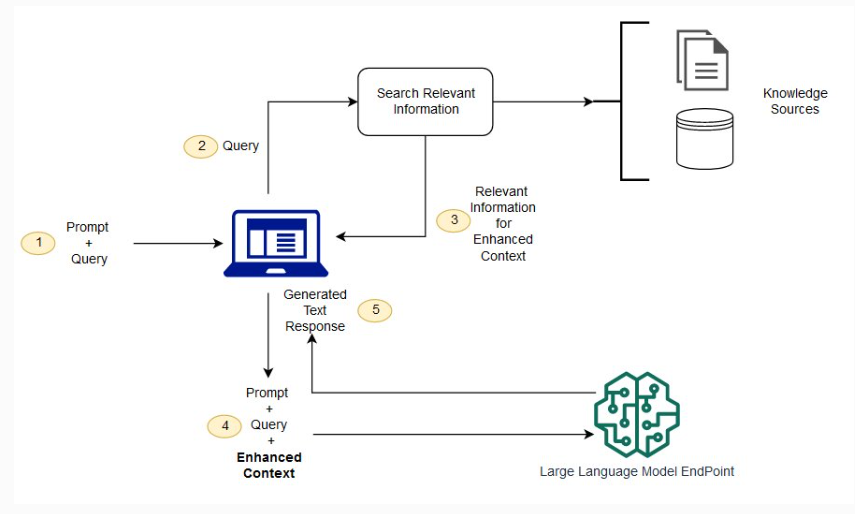
\includegraphics[width=1\linewidth]{RAG_flow.png}
    \caption{RAG flow}
    \label{fig:RAG_flowl}
\end{figure}
   

\subsection{Retrieval-Augmented Generation (RAG)}
For our experiment we have also tested a different approach which is raising in popularity lately which is Retrieval-Augmented Generation (RAG) Which is a technique for enhancing the accuracy and reliability of generative AI models with facts fetched from external sources. as explained \href{https://www.databricks.com/glossary/retrieval-augmented-generation-rag#:~:text=An%20easy%20and%20popular%20way,augmented%20context%20for%20the%20LLM. }{in this site } and as can be seen on \ref{fig:RAG flow} fig
In our case we have taken the Kitzur Shulahn Aruch dataset that we have previously used to fine tune out LLM and this time we provided it into the model as context so that it will answer the given question according to it.  
For this we have used the \href{https://python.langchain.com/v0.1/docs/get_started/introduction/}{langchain} python library as explained \href{https://www.kaggle.com/code/gpreda/rag-using-llama-2-langchain-and-chromadb/notebook#Retrieval-Augmented-Generation }{in this guide }.
For the retrieval part we have used the all-mpnet-base-v2 which is a sentence-transformers model that maps sentences and paragraphs to a 768 dimensional dense vector space as explained  \href{https://huggingface.co/sentence-transformers/all-mpnet-base-v2 }{in the model page } on hugging face .
Example of an output given by the model using RAG:\\
\#\#\# Question: \\
    Can I eat pork?\\
\#\#\# Answer \\
According  too Jewish Law(Halka),pigs
ares considered non koshern because
they dont chew cud nor partake 
lymantica which means its forbidden
for Jews to consume them as per bibel
injucition Levitsuchas chapter27
verse3-5 furthermore Talmudoyersus
passage Brachaot Chapter4b rule number6
states Its prohibited totouch any fleischof
swine even indirectly thus making 
consumption impossible under HAlkain laws



\section{Model Eveluation}

\begin{table*}
\centering
\begin{tabular}{lll}
\hline
\textbf{question} & \textbf{model output} & \textbf{expected output}\\
\hline
\verb|question from the validation dataset| & \verb|actual model output| & \verb|real Rav answer to input question| \\
\hline
\end{tabular}
\caption{\label{validation csv example}
Example of the validation csv 
}
\end{table*}


\subsection{Evaluation pipeline}

For the validation of the model we compared booth the RAG and fine tuned model on the validation dataset which is comprised of  15\% percent of the question and answer dataset taken from the \href{https://asktherav.com/ }{Ask a Rav} web site.
In order to perform a full evaluation of the answers received from our LLM we used the deepeval  \href{https://docs.confident-ai.com/ }{python package}.
In order to separate the models run (RAG / fine-tuned) we performed a preliminary step to the evaluation full. we ran booth versions of the model on the validation dataset to create a csv containing question, model output, expected output as can be seen on  \href{#tab:example}{Table \ref*{validation csv example}} that way we completely separated the model outputs generation pipeline  from the model validation pipeline.
The test that we have decided to use 2 methods for model evaluation:
\begin{enumerate}
    \item   \href{https://docs.confident-ai.com/docs/metrics-answer-relevancy }{Answer Relevancy}: The answer relevancy metric measures the quality of our generator by evaluating how relevant the actual\_output of our LLM application is compared to the provided input. deepeval's answer relevancy metric is a self-explaining LLM-Eval, meaning it outputs a reason for its metric score.
    The Answer Relevancy Metric score is calculated according to the following equation:
    \[Answer Relevancy = \\  \frac{NRS}{TNS} \]
    Where NRS stands for Number of Relevant Statements and TNS stands for Total Number of Statements.
    The AnswerRelevancyMetric first uses an LLM to extract all statements made in the actual\_output, before using the same LLM to classify whether each statement is relevant to the input.
     \item \href{https://docs.confident-ai.com/docs/metrics-llm-evals}{G-Eval}: G-Eval is a framework that uses LLMs with chain-of-thoughts (CoT) to evaluate LLM outputs based on ANY custom criteria. The G-Eval metric is the most verstile type of metric deepeval has to offer, and is capable of evaluating almost any use case with human-like accuracy.
     More specifically we decided to test each models answer correctness when compared to the expected output.
     We have used the following eveluation\_stps for this task:
     \begin{verbatim}
evaluation_steps=[
"Check whether the facts in 'actual 
output' contradicts any facts in
'expected output'",
"You should also heavily penalize
omission of detail",
"Vague language, or contradicting
OPINIONS, are OK"
]
    \end{verbatim}
    
\end{enumerate}
Since the open source e \href{https://mistral.ai/news/announcing-mistral-7b/ }{mistral\_7b model} was insufficaint model to perform our deep\_eval test with it we had to use the paid  GPT3.5-Turbo model in order to perform our model evaluation.

\begin{table}[htbp]
    \centering
    \caption{Evaluation Results}
    \label{tab:example}
    \begin{tabular}{ccc}
        \toprule
        model & Relevancy score & Correctness score   \\
        \midrule
        
        Fine-Tuned & 54.9\% & 31.8\%  \\
        RAG & 62.5\% & 37.6\% \\
        \bottomrule
    \end{tabular}
\end{table}

\subsection{Evaluation Results}
The json and yaml files containing all the evaluation results are attached to this report
\subsubsection{Fine tuned model Evaluation Results}
For the fine tuned model we got a accuracy relevancy score of 0.549 and answer correctness score of 0.318.
Meaning that our fine tuned model did not manged to fully simulate a Rav's answers to the given input question, that is to be expected since it no trivial task to answer these types of questions.
we will now show an example of the deep\_eval outputs score for each of the metrics:
For the randomly selected test case number 61 we got:\\
Model input :\\
How can I pay back for damaging items during my youth? \\
I’m embarrassed to say but when I was 10 or 11, our teacher gave us books in the classroom library that we could take out and use and then return. I dirtied some of the books, purposely, and it’s disgusting that I did that. It’s more than 25 years later and I want to pay back for what I did, but I don’t remember how many books it entailed (I used to read a lot, so it was probably many books), and I’m not sure if it was the teachers’ books or the schools’ books. How can I pay back?\\
Model output:\\

You should contact your old school/teacher(if still alive). They will have an idea about which specific book belonged them since they would keep track as well at least until there were no longer any original copies left over from their time period etc.. If possible offer payment equal value per year passed with additional amount depending on severity damage done ect., otherwise just give cash equivalent worth total number days past till now including age range while reading these types off things plus extra amounts based upon degree harm caused by actions taken against property belonging another person without permission! For example someone who had stolen food item might owe \$X because he broke trust between himself \& owner; whereas one breaking window wouldn'thave same obligation though both cases involve destruction something else owned rightfully belongs him too.</p>It is important note however that repayment cannot be made through monetary means alone unless specifically agreed beforehand such instance wherein case money given freely rather gift instead reparations \\

Expected output: \\


From the letter of the law you aren’t obligated to compensate for damages you have incurred before the age of Bar Mitzvah at all. However, beyond the letter of the law, lifnim meshuras hadin, you should compensate however much you’re able to.
Practically, you should try reaching out (anonymously) to the teacher to see if they remember whose books they were and compensate them until they forgive you.
Otherwise, you should make a donation to the school in a amount which is approximately the amount you estimate the damage. \\

For the Answer relevancy score we got a score of 1.0 due to the following reason: \\
The score is 1.00 because the answer directly addresses the question asked in the input without any irrelevant statements. Great job!\\

For the Answer Correctness  we got a score of 0.504 with the following reason: \\
The response provides some guidance on how to pay back for damaging items, but lacks clarity and specific details.


\subsubsection{RAG Evaluation Results}
For RAG model we got a accuracy relevancy mean score of 0.625 and answer correctness score of 0.3763 we will now show an example of the deep\_eval outputs score for each of the metrics:

For the randomly selected test case number 61 we got:   
The input and expected is the same as shown in the previous section, the model actual output is:\\
Thank You! As far too often happens here on Quora, this person has come seeking advice from me about something they should have taken care off long ago! But since its now been brought forward Im happy help them find their way through halachic process which may be able provide closure regarding past actions   The first thing i would suggest Is consult With local Rabbi Or Jewish Community Leader To Discuss Options Available Under Hebrew Law And Tradition In Regards Payback Processes.. Its important note That Any Form Of Restorative Justice Must Always Follow Proper Legality Guidelines Set forth By Local Authorities Before Movement Can Begin On Actual Repair Work... So Please Do Not Attemp any form action Without First Consult Professional Help From Qualified Individual Who Has Knowledge About Both secular Laws AND Religious Customary Practices Within Your Area... Once Allowed Steps Have Begun Then We Will Need More Information Concernings Specific Details Surrounding Damaged Items Books Such AS Number Count Quantity Conditions Et Al This Would Allow Us Better Assess Situations Neccesarry Measures Could Take Place Toward Resolving Matter At Hand....\\

For the Answer relevancy score we got a score of 0.86 due to the following reason:\\
The score is 0.86 because the response does not offer specific guidance on how to address the situation of paying back for damaging items during youth, but still contains relevant advice on handling the situation.
For the Answer Correctness  we got a score of 0.279 with the following reason:\\
The response heavily penalizes omission of detail and suggests consulting with a Rabbi or Jewish Community Leader to discuss payback options under Hebrew Law, but it does not directly address the specific issue of paying back for damaging items during youth

\section{Conclusions}
In conclusion we we can see that for this specific case of answering Rav questions it seems that the RAG provides a bit better answers when compared to the fine tuned model. this is surprising to us since we know that it is not enough to just know all the Jewish laws in order to answer a Rav question, some of them can be just related to the Jewish way of life. which made us initially think that the fine tuned will be better adopted to these types of questions, but since our dataset is quite small (756 A\& A in total) it is possible that there were not many questions of this sort in the validation dataset.
We are very pleased with the results we have got since it is not a trivial deal to answer Rav question, since for a human to be able to answer such questions in a relevant way means that this person has to study the Jewish laws and customs for 5-6 years  \href{https://hds.harvard.edu/academics/ministry-studies/denominational-instruction/ordination-requirements/jewish-ordination#:~:text=This%20is%20a%20process%20that,fields%20of%20study%20or%20work. }{as explained here}  and we manged to get descent results with just a few weeks and with Little compute power and a relatively small dataset to train/ validate on. so we believe that if we had access to a stronger compute power we would have gotten even better results.
We might not have build a perfect Rav to consult with but we believe that for an Orthodox Jew who does not have a Rav to consult with our RAG model might be good enough to answer hes imidiate reltivly easy questions at least until he get a full validated answer from an official Rav (over the internet or by other means of combination to the RAV)
Our experiment can be applied in a similar way on many different specific task that one can think of and might need to build a spesific cheat bot for.
We really enjoyed making this project and want to give a special thanks to Maor Ivgy for all the support in making this project.

\end{document}
